% Plantilla simple para tareas de la Licenciatura en Física
% Fer Flores - Universidad de Guadalajara - Noviembre 2023

%%%%%%%%%%%%%%%%%%%%%%%%%%%%%%%%%%%%%%%%%%-PREÁMBULO-%%%%%%%%%%%%%%%%%%%%%%%%%%%%%%%%%%%%%%%%%%

% Paqueterías

\documentclass{assignment}
\usepackage[pdftex]{graphicx} % FIGURAS
\usepackage{xcolor}
\definecolor{LightGray}{gray}{0.95}
\usepackage{fancyvrb, minted} % CÓDIGO
\usepackage[letterpaper, margin = 2.5cm]{geometry} % TAMAÑO DE PÁGINA Y MÁRGENES
\usepackage[T1]{fontenc} % Importante para acentos automáticos y símbolos de escritura
\usepackage{amsmath, amsfonts, amssymb} % Ecuaciones, caracteres y símbolos especiales
\usepackage{hyperref, url}  % Links y Hyperlinks en el documento
\usepackage{fancyhdr}

%-----------------------------------------ETIQUETAS--------------------------------------------

\student{Lyndsey Gu}                             % NOMBRE
\date{\today}                                   % Fecha (Modifica a DD/MM/AAAA)

\courselabel{lyndsey.gu@gmail.com}          % CARERA (Física, la mejor carrera)
\exercisesheet{lyndskg}         % LA PODEROSÍSIMA

\exercisesheet{Implementing Black-Scholes Model}{black-scholes-cpp}     % NÚMERO Y TÍTULO DE LA TAREA

\school{Department of Electrical Engineering and Computer Science}          % CARERA (Física, la mejor carrera)
\university{University of Michigan}         % LA PODEROSÍSIMA


%%%%%%%%%%%%%%%%%%%%%%%%%%%%%%%%%%%%%%%%%%-DOCUMENTO-%%%%%%%%%%%%%%%%%%%%%%%%%%%%%%%%%%%%%%%%%%%%

\begin{document}

%-----------------------------------------------------------------------------------------------
\begin{problem}

\section{Right off the bat...}

\noindent To start, I studied the Black-Scholes model and the mathematical foundations of option pricing. 
\begin{itemize}
    \item Implement the necessary formulas and calculations, paying attention to accuracy and efficiency. 
    \item Validate your implementation by comparing results with established pricing models.
\end{itemize}


\begin{itemize}
    \item Study the fundamentals of option pricing, including the Black-Scholes model. 
    \item Understand the required formulas and their implementation. Start by implementing the basic components and gradually build upon them to create a functional option pricing program.
    \item Study the Black-Scholes model and the underlying mathematical concepts.
\end{itemize}
    

\noindent Implement the necessary formulas for option pricing, including calculations for Greeks (Delta, Gamma, Theta, etc.).

\noindent Design and implement a user-friendly interface for inputting option parameters and obtaining pricing results.

\subsection{Preliminary Considerations}

\noindent Initial considerations and qualms when embarking on this project.

\begin{enumerate}
    \item Understand the theoretical and real-world applications of the Black-Scholes formula. 
    \item Consider doing back-testing... WRITING IN C\(sharp\) FIRST.
    \item Begin devising a function to calculate option prices based on the Black-Scholes formula — creating methods and private member variables.
    \item Try to determine the best (i.e. most accurate) approximation for the normal CDF distribution, and write a function for that.
    \item Deal with getter/setter functions for all of the member variables — should it be from a static .CSV file or should I try to wield real-time market data feeds?
\end{enumerate}

\subsubsection*{\underline{Oh no... math...}}

\begin{itemize}
    \item Use $mu = 0$, $theta = 1$ for the general Gaussian PDF.
    \item If you have access to a standard math library, you will most probably find the error function $erf$ and maybe the complementary function $$erfc(x) = 1 - erf(x)$$ which nowadays are used to compute the normal CDF, i.e. the A and S function $P(x)$ s.t. 
    \begin{align*}
        P(x) & = \dfrac{1}{\sqrt{2\pi}} \int_{-\infty}^{x} (e^{-t^2 / 2}) \, dt \\
             & = \int_{-\infty}^{x} Z(t) \  dt \\
             & = \dfrac{1}{2} (1 + erf(\dfrac{x}{\sqrt{2}}) \\
             & = \dfrac{1}{2} \ erfc \ (- \dfrac{x}{\sqrt{2}}) \\
    \end{align*}
\end{itemize}


\begin{figure}
    \centering
    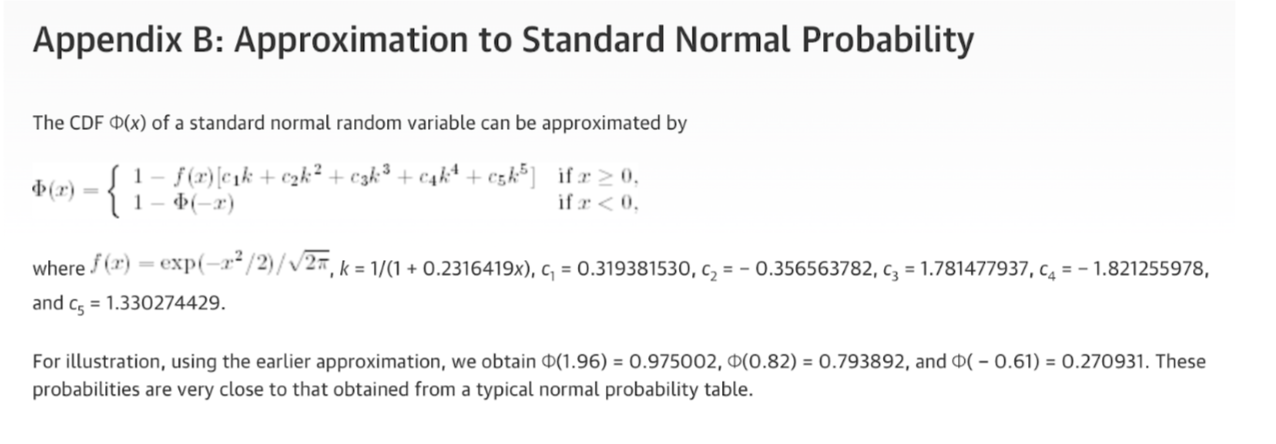
\includegraphics[width=0.8\linewidth]{Screenshot 2024-01-07 at 4.51.06 AM.png}
    \label{fig:enter-label}
\end{figure}


\subsubsection*{\underline{Scouting for open-source, real-time market stream APIs}}

\noindent Want to use real-time data feeds; faced roadblock as most financial data providers or exchanges that offer real-time services require obtaining credentials and/or API keys and additional charges. \\

\noindent TD Ameritrade only has an open-source Git repo/package written in Rust with Python co-routines — bad for C++ project. \\\\\

\noindent\textbf{Exploring other free real-time market-data feed Finance APIs:} \\\\
\noindent \textit{Note}: Based on reviews, financial and other user accessibility concerns, UI/UX, and numerous other factors, I narrowed it down to Alpaca, AlphaVantage, or Yahoo Finance. \
\begin{itemize}
    \item Tiingo
    \item polygon.io
    \item Financial marketing prep
    \item Tardis.dev
    \item AlphaVantage
    \begin{itemize}
        \item Alpha Vantage is a financial data provider that offers free and paid APIs for accessing various financial data, including real-time and historical stock prices, technical indicators, fundamental data, and more. \
        \item They have a generous free plan that allows for a high number of API calls per minute. \
        \item Alpha Vantage is a good choice if you need a wide range of financial data beyond just stock prices and want to have flexibility in accessing and analyzing the data. \ 
    \end{itemize}
    \item coinapi.io
    \item kaiko
    \item nomics
    \item tradier
    \item amberdata.io
    \item brave new coin
    \item xignite
    \item intrinio
    \item iexcloud.io
    \item eodhd
    \item finnhub.io
    \item marketstack
    \item twelvedata
    \item IQfeed
    \item IBKR APIs
    \item fmpcloud.io
    \item Alpaca
    \begin{itemize}
        \item Alpaca is a technology-driven brokerage that offers a powerful API for accessing market data and executing trades. \
        \item They provide a wide range of real-time and historical market data, including equities, options, and crypto. \
        \item Alpaca's API is developer-friendly and offers a free data plan with limited access. They also have premium plans for more extensive data needs. \
        \item Consider Alpaca if you prefer a modern API and are interested in exploring more advanced trading functionalities in the future. \ 
    \end{itemize}
    \item StockData
    \item Yahoo Finance API 
    \begin{itemize}
        \item https://github.com/foxadb/yahoo-finance 
        \item Yahoo Finance provides financial news, data, and stock prices. 
        \item They offer a free API that allows you to access a variety of financial data, including historical stock prices and some basic company information. 
        \item Yahoo Finance is a good option if you primarily need historical stock prices for your backtesting purposes.
    \end{itemize}
\end{itemize} 

\subsubsection*{\underline{Optimization}}

\begin{itemize}
    \item Utilize numerical libraries: Consider using numerical libraries, such as the Intel Math Kernel Library (MKL) or the GNU Scientific Library (GSL), which provide optimized implementations of mathematical functions and numerical algorithms. 
    \begin{itemize}
        \item These libraries can help improve the performance of your calculations and provide more accurate results.
    \end{itemize}
    \item Parallelize computations: If your algorithm involves performing calculations on large datasets or performing multiple calculations simultaneously, you can consider parallelizing your computations.
    Utilize parallel programming techniques, such as multi-threading or distributed computing, to take advantage of multiple cores or distributed systems. 
    Libraries like OpenMP or Intel TBB can assist you in parallelizing your code. 
    \item Optimize memory usage: Pay attention to memory allocation and deallocation in your code. 
    Efficient memory management, such as using appropriate data structures, minimizing unnecessary copies or allocations, and utilizing memory pools, can improve the performance of your algorithm.
    \item Compiler optimizations: Take advantage of compiler optimizations to improve the execution speed of your code. 
    Enable compiler optimizations, such as loop unrolling, function inlining, and vectorization, to enhance the performance of your algorithm. 
    Consult your compiler's documentation or explore compiler flags to enable these optimizations.
    \item Algorithmic optimizations: Consider exploring alternative numerical algorithms or optimization techniques that can improve the efficiency of your calculations. 
    Look into numerical methods that provide faster convergence or reduced computational complexity for specific scenarios.
    \item Profiling and benchmarking: Use profiling and benchmarking tools to identify performance bottlenecks in your code. 
    These tools can help you understand where your algorithm spends most of its time and guide your optimization efforts.
\end{itemize}

\noindent \textit{Keep in mind that optimization should be done judiciously, and it's important to balance performance improvements with code readability, maintainability, and correctness. Measure the impact of optimizations through profiling and testing to ensure they deliver the desired performance gains without introducing unintended side effects.
Remember to adapt these suggestions to the specific requirements of the Black-Scholes Model implementation and consider the trade-offs associated with each optimization technique.
} \\\\



\subsubsection*{\underline{Backtesting}}

\noindent Backtesting is a valuable practice in the development of trading strategies, especially in the context of high-frequency trading (HFT). Backtesting involves simulating and evaluating the performance of a trading strategy using historical market data. \\
While backtesting is not mandatory, it is highly recommended for several reasons:
\begin{itemize}
    \item Performance Evaluation: Backtesting allows you to assess the effectiveness of your trading strategy by simulating its performance on historical data. It helps you understand how the strategy would have performed in real-world conditions and provides insights into its profitability, risk management, and overall performance.
    \item Strategy Refinement: Backtesting provides an opportunity to refine and optimize your trading strategy. By analyzing the results of backtests, you can identify strengths and weaknesses, make necessary adjustments, and fine-tune your strategy to improve its performance.
    \item Risk Management: Backtesting helps you evaluate the risk associated with your trading strategy. By analyzing historical data, you can assess the drawdowns, volatility, and potential losses that your strategy may experience in different market conditions. This information is crucial for risk management and position sizing.
    \item Confidence Building: Backtesting allows you to gain confidence in your trading strategy before deploying it in real-time trading. By demonstrating positive results over a significant period of historical data, you can develop trust in your strategy and its ability to generate profits.
\end{itemize}

\noindent \textit{While backtesting is beneficial, it's important to note that it has its limitations. Backtesting relies on historical data, and the future market conditions may not precisely mirror the past. Therefore, it's essential to interpret backtest results with caution and consider the potential impact of changing market dynamics.}\\\\

To perform backtesting, you'll need historical market data, a well-defined trading strategy, and the ability to implement the strategy in code. There are various tools and libraries available that can assist you in conducting backtests, such as popular platforms like MetaTrader, backtesting frameworks like Backtrader, or building custom solutions using programming languages like Python, C++, or R.\\\\
Overall, while backtesting is not strictly necessary, it is highly recommended as an integral part of developing and evaluating trading strategies in the context of HFT. It can provide valuable insights, help you refine your strategies, and improve your overall trading performance.


\subsubsection*{How to backtest?}
\noindent To backtest your algorithm, you would follow these general steps:\\
\begin{itemize}
    \item Obtain historical market data: Acquire historical price data for the relevant financial instruments you are trading. You can find such data from various sources, such as financial data providers or online platforms that offer historical market data.
    \item Implement the backtesting framework: Create a separate module or set of functions to handle the backtesting process. This module should include components such as data loading, strategy execution, performance metrics calculation, and result analysis.
    \item Load historical market data: Import the historical market data into your backtesting framework. This data will serve as the input for your algorithm during the backtesting process.
    \item Implement the strategy execution logic: Translate your algorithm from C# to the desired programming language (in this case, C++). Replicate the logic and calculations used in the CSharp implementation.
    \item Simulate trades: Iterate through the historical data, step by step, and simulate trades based on the trading signals generated by your algorithm. Keep track of your portfolio's equity, positions, and other relevant variables.
    \item Calculate performance metrics: Measure the performance of your algorithm by calculating various metrics such as returns, drawdowns, Sharpe ratio, and other risk-adjusted measures.
    \item Analyze the results: Evaluate the backtesting results to gain insights into the performance of your algorithm. Identify strengths, weaknesses, and areas for improvement. This analysis can help you refine your strategy and make necessary adjustments.
\end{itemize}

\noindent Once you have completed the backtesting process and are satisfied with the results, you can then proceed with converting your algorithm from CSharp to C++.\\
This involves rewriting the code, replicating the logic, calculations, and data structures in C++.\\
You can refer to your CSharp implementation as a reference and make the necessary adjustments to ensure it functions correctly in the C++ environment.\\\\
Keep in mind that converting the code from one language to another may require considering language-specific differences, libraries, and syntax.\\\\
Additionally, you may need to adapt any external dependencies or APIs used in your CSharp implementation to their equivalent counterparts in C++.\\\\
It's worth noting that backtesting is an essential step in algorithmic trading development, as it allows you to assess the historical performance of your strategy.\\\\
It helps you gain confidence in the strategy's robustness and reliability before deploying it in live trading.\\\\

\begin{figure}
    \centering
    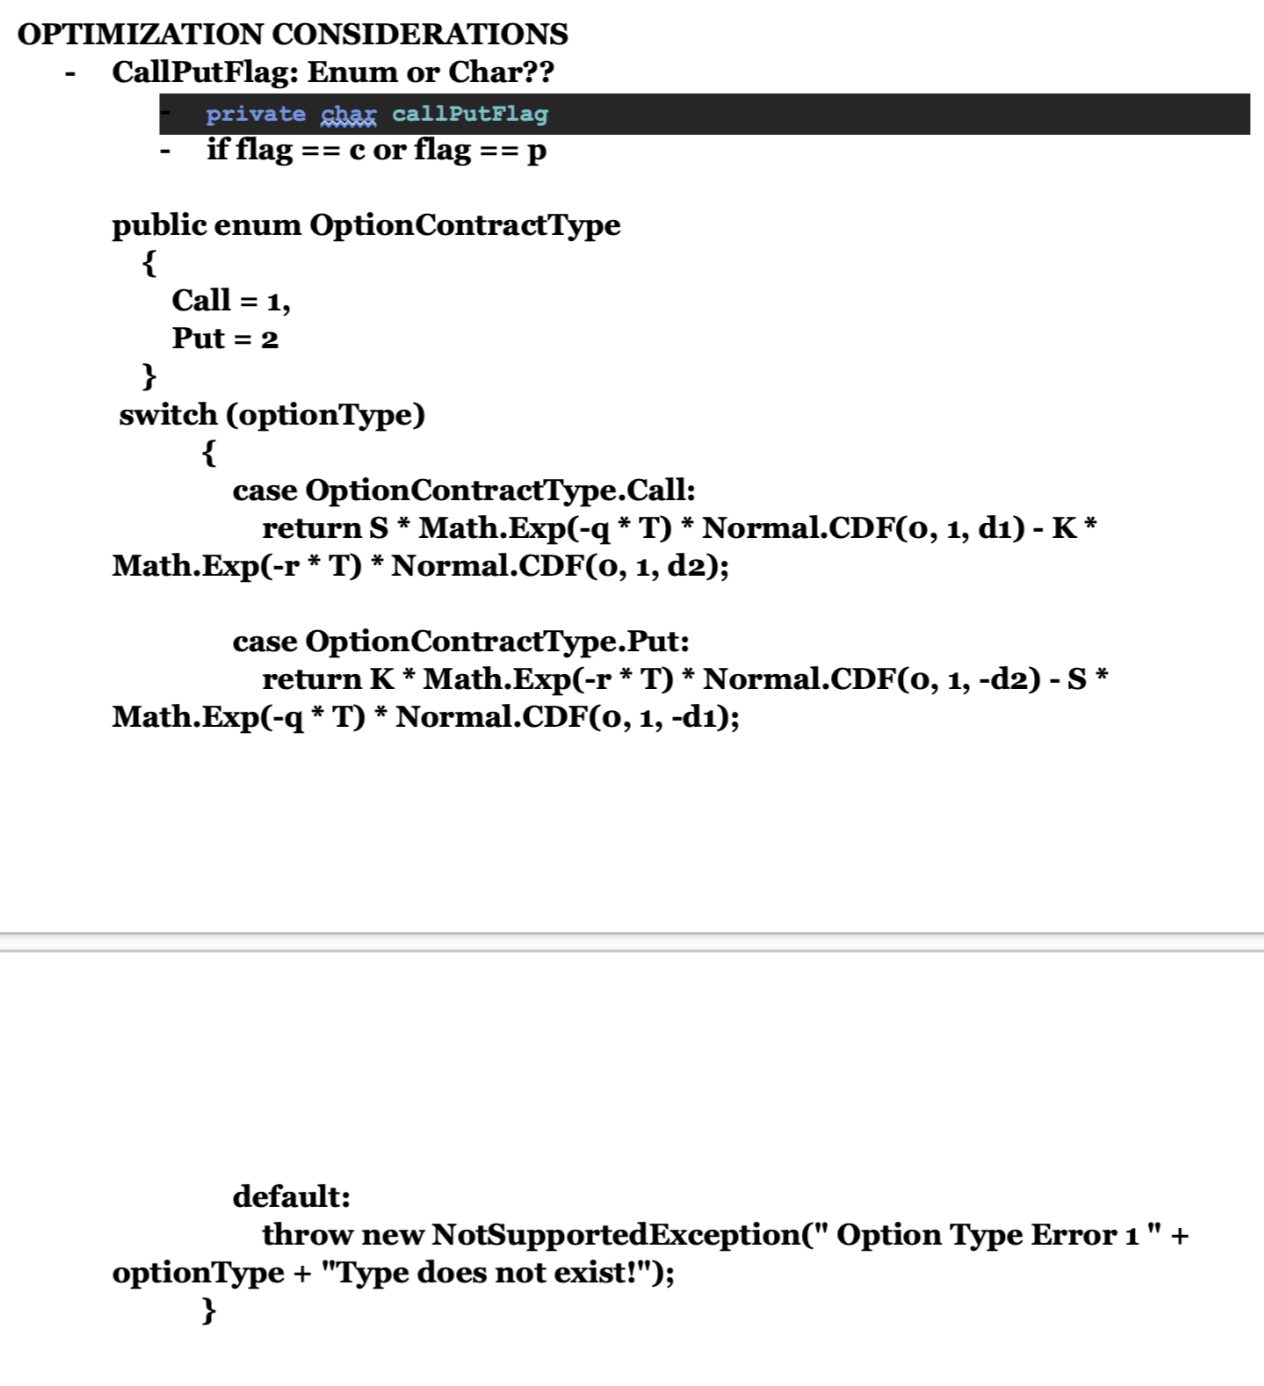
\includegraphics[width=0.85\linewidth]{Screenshot 2024-01-07 at 5.23.56 AM.png}
    \label{fig:enter-label}
\end{figure}

\end{problem}
%---------------------------------------------------------------------------------------------
% \begin{problem}

% \section{Segundo Problema}

% \noindent
    
% \end{problem}
%---------------------------------------------------------------------------------------------



%--------------------------------------BIBLIOGRAFIA-------------------------------------------

\newpage

\nocite{*} % Agrega las referencias aunque no las hayas citado directamente

\bibliographystyle{unsrt}    % ESTILO DE BIBLIOGRAFÍA (Recomendados: abbrv, ieeetr, apalike, unsrt)
\bibliography{refs}     % REFERENCIAS EN ARCHIVO SEPARADO


\end{document}
